% ++++++++++++ Controller PSoC Master klassen ++++++++++++++
\subsubsection{Boundary-klasse: DistanceSensor}

Denne klasse har til formål at styre kommunikation mellem Pi og afstandssensorer, der er valgt at benytte I2C-kommunikation til dette. De 4 afstandssensorer er navngivet efter deres respektive placering på bilen: ''Front Left'' = ''FL'', ''Front Left'' = ''FL'' ''Front Left'' = ''RL'', ''Rear Right'' = ''RR''. 

\begin{figure}[h]
\centering
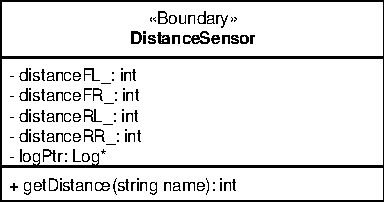
\includegraphics[]{../fig/diagrammer/bil/cd_distancesensor.pdf}
\caption{Klassebeskrivelse af boundary-klassen DistanceSensor}
\label{fig:cd_distancesensor}
\end{figure}

\textbf{Attributter}

\begin{table}[h]
	\begin{tabularx}{\textwidth}{| Z | Z | L{10cm} |} \hline
		Navn & Type & Beskrivelse \\\hline
		\texttt{distanceFL\_} & \texttt{int} 		& Midlertidig variabel der indeholder afstanden fra forreste venstre afstandssensor.\\\hline
		\texttt{distanceFR\_} & \texttt{int} 		& Midlertidig variabel der indeholder afstanden fra forreste højre afstandssensor.	\\\hline
		\texttt{distanceRL\_} & \texttt{int} 		& Midlertidig variabel der indeholder afstanden fra bagerste venstre afstandssensor \\\hline
		\texttt{distanceRR\_} & \texttt{int} 		& Midlertidig variabel der indeholder afstanden fra bagerste højre afstandssensor.	\\\hline
		\texttt{logPtr\_} 	 & \texttt{log*} 		& Pointer til at skrive i den globale Log											\\\hline
	\end{tabularx}
	\caption{Attributter for klassen DistanceSensor}
	\label{table:attr_distancesensor}
\end{table}
\clearpage

\textbf{Metoder}

\begin{table}[h]
	\begin{tabularx}{\textwidth}{| L{2.5 cm} | Z |} \hline
		Prototype 	& \texttt{int getDistance(string name)} \\\hline
		Parametre 	& \texttt{name} \newline Navnet på den sensor som der skal læses fra. Kan rumme én af fire muligheder "FL", "FR", "RL" og "RR". \\\hline
		Returværdi 	& \texttt{int} \newline Seneste afstandsmåling for den pågældende sensor. Værdien er angivet i cm. \\\hline
	\end{tabularx}
	\caption{Metodebeskrivelse for \texttt{getDistance}}
	\label{table:met_getdistance}
\end{table}
\clearpage


% /////////////////////////////////////////////////////////////////////////////
%					SW design af distanceSensor
% ////////////////////////////////////////////////////////////////////////////


Afstandssensorene leveres formonteret på print hvor benene fra IC'en er trukket til harwinpins som let kan tilgås. Til kommunikationen med sensoren benyttes følgende 4 linjer: 

\begin{itemize}
	\item pin 7: VCC: Forsyning
	\item pin 6: GND: Reference
	\item pin 5: SCL: Clock
	\item pin 4: SDA: Data
\end{itemize}

Data kommunikeres på SDA-linjen med reference til GND,  SCL styrer clocken.
Der benyttes de hardcodede default adresser til de 4 sensorer, disser er som følger: 

\begin{table}[h]\centering
	\begin{tabular}{| l | l |} \hline
		\textbf{Sensor} 	& \textbf{Adresse}  \\\hline
		FL 					& \texttt{0x70} 	\\\hline
		FR 					& \texttt{0x71} 	\\\hline
		RL 					& \texttt{0x73} 	\\\hline
		RR 					& \texttt{0x76} 	\\\hline
	\end{tabular}
	\caption{Adresser på afstandssensorer}
	\label{table:adr_afstandssensorer}
\end{table}

For at kunne benytte sensorerne skal der sendes en række kommandoer til hver enkelt sensor. Disse kommandoer følger fremgangsmåden herunder:

\begin{enumerate}
  \item \textit{write}-mode-Kommando sendes til den given sensoradresse.
  \item Der kan skrives til sensoradressen
  \item \textit{read}-mode-Kommando sendes til den given sensoradresse.
  \item Der kan skrives fra sensoradressen
\end{enumerate}

Alle \textit{write}- eller \textit{read}-kommandoer foregår altså som koblinger af 2 kommandoer, én hvor der sætte ''mode'' og til at foretage en given kommando. Derudover kommer databladets anbefalede 100ms til at foretage en Range-reading inden den aflæses.

Følgende kommandoer er benyttet til at skrive og læse fra sensorerne: 

\begin{table}[h]\centering
	\begin{tabular}{| l | l |} \hline
		\textbf{Kommando} & \textbf{Adresse}	\\\hline
		FLwrite 		  & 0xE0				\\\hline
		FRwrite 		  & 0xE2				\\\hline
		RLwrite 		  & 0xE6				\\\hline
		RRwrite 		  & 0xEC				\\\hline
		FLread  		  & 0xE1				\\\hline
		FRread  		  & 0xE4				\\\hline
		RLread  		  & 0xE7				\\\hline
		RRread  		  & 0xED				\\\hline
		StartReading	  & 0x51				\\\hline
	\end{tabular}
	\caption{\textit{read/write}-kommandoer til afstandssensorer}
	\label{table:adr_afstandssensorer_kommadoer}
\end{table}
